% *** Authors should verify (and, if needed, correct) their LaTeX system  ***
% *** with the testflow diagnostic prior to trusting their LaTeX platform ***
% *** with production work. IEEE's font choices can trigger bugs that do  ***
% *** not appear when using other class files.                            ***
% The testflow support page is at:
% http://www.michaelshell.org/tex/testflow/


%%*************************************************************************
%% Legal Notice:
%% This code is offered as-is without any warranty either expressed or
%% implied; without even the implied warranty of MERCHANTABILITY or
%% FITNESS FOR A PARTICULAR PURPOSE!
%% User assumes all risk.
%% In no event shall IEEE or any contributor to this code be liable for
%% any damages or losses, including, but not limited to, incidental,
%% consequential, or any other damages, resulting from the use or misuse
%% of any information contained here.
%%
%% All comments are the opinions of their respective authors and are not
%% necessarily endorsed by the IEEE.
%%
%% This work is distributed under the LaTeX Project Public License (LPPL)
%% ( http://www.latex-project.org/ ) version 1.3, and may be freely used,
%% distributed and modified. A copy of the LPPL, version 1.3, is included
%% in the base LaTeX documentation of all distributions of LaTeX released
%% 2003/12/01 or later.
%% Retain all contribution notices and credits.
%% ** Modified files should be clearly indicated as such, including  **
%% ** renaming them and changing author support contact information. **
%%
%% File list of work: IEEEtran.cls, New_IEEEtran_how-to.pdf, bare_jrnl_new_sample4.tex,
%%*************************************************************************
\PassOptionsToPackage{unicode}{hyperref}
\PassOptionsToPackage{hyphens}{url}
\PassOptionsToPackage{dvipsnames,svgnames,x11names}{xcolor}
% Note that the a4paper option is mainly intended so that authors in
% countries using A4 can easily print to A4 and see how their papers will
% look in print - the typesetting of the document will not typically be
% affected with changes in paper size (but the bottom and side margins will).
% Use the testflow package mentioned above to verify correct handling of
% both paper sizes by the user's LaTeX system.
%
% Also note that the "draftcls" or "draftclsnofoot", not "draft", option
% should be used if it is desired that the figures are to be displayed in
% draft mode.
%
\documentclass[
  journal,
]{IEEEtran}%
% If IEEEtran.cls has not been installed into the LaTeX system files,
% manually specify the path to it like:
% \documentclass[journal]{../sty/IEEEtran}
\usepackage[cmex10]{amsmath}
\usepackage{amssymb}
\usepackage{iftex}
\ifPDFTeX
  \usepackage[T1]{fontenc}
  \usepackage[utf8]{inputenc}
  \usepackage{textcomp} % provide euro and other symbols
\else % if luatex or xetex
  \usepackage{unicode-math} % this also loads fontspec
  \defaultfontfeatures{Scale=MatchLowercase}
  \defaultfontfeatures[\rmfamily]{Ligatures=TeX,Scale=1}
\fi
%\usepackage{lmodern}
\ifPDFTeX\else
\fi
% Use upquote if available, for straight quotes in verbatim environments
\IfFileExists{upquote.sty}{\usepackage{upquote}}{}
\IfFileExists{microtype.sty}{% use microtype if available
  \usepackage[]{microtype}
  \UseMicrotypeSet[protrusion]{basicmath} % disable protrusion for tt fonts
}{}
\makeatletter
\parindent    1.0em
\ifCLASSOPTIONcompsoc
  \parindent    1.5em
\fi
\makeatother
\usepackage{xcolor}
\setlength{\emergencystretch}{3em} % prevent overfull lines

\setcounter{secnumdepth}{5}
% Make \paragraph and \subparagraph free-standing
\ifx\paragraph\undefined\else
  \let\oldparagraph\paragraph
  \renewcommand{\paragraph}[1]{\oldparagraph{#1}\mbox{}}
\fi
\ifx\subparagraph\undefined\else
  \let\oldsubparagraph\subparagraph
  \renewcommand{\subparagraph}[1]{\oldsubparagraph{#1}\mbox{}}
\fi

\usepackage{color}
\usepackage{fancyvrb}
\newcommand{\VerbBar}{|}
\newcommand{\VERB}{\Verb[commandchars=\\\{\}]}
\DefineVerbatimEnvironment{Highlighting}{Verbatim}{commandchars=\\\{\}}
% Add ',fontsize=\small' for more characters per line
\usepackage{framed}
\definecolor{shadecolor}{RGB}{241,243,245}
\newenvironment{Shaded}{\begin{snugshade}}{\end{snugshade}}
\newcommand{\AlertTok}[1]{\textcolor[rgb]{0.68,0.00,0.00}{#1}}
\newcommand{\AnnotationTok}[1]{\textcolor[rgb]{0.37,0.37,0.37}{#1}}
\newcommand{\AttributeTok}[1]{\textcolor[rgb]{0.40,0.45,0.13}{#1}}
\newcommand{\BaseNTok}[1]{\textcolor[rgb]{0.68,0.00,0.00}{#1}}
\newcommand{\BuiltInTok}[1]{\textcolor[rgb]{0.00,0.23,0.31}{#1}}
\newcommand{\CharTok}[1]{\textcolor[rgb]{0.13,0.47,0.30}{#1}}
\newcommand{\CommentTok}[1]{\textcolor[rgb]{0.37,0.37,0.37}{#1}}
\newcommand{\CommentVarTok}[1]{\textcolor[rgb]{0.37,0.37,0.37}{\textit{#1}}}
\newcommand{\ConstantTok}[1]{\textcolor[rgb]{0.56,0.35,0.01}{#1}}
\newcommand{\ControlFlowTok}[1]{\textcolor[rgb]{0.00,0.23,0.31}{\textbf{#1}}}
\newcommand{\DataTypeTok}[1]{\textcolor[rgb]{0.68,0.00,0.00}{#1}}
\newcommand{\DecValTok}[1]{\textcolor[rgb]{0.68,0.00,0.00}{#1}}
\newcommand{\DocumentationTok}[1]{\textcolor[rgb]{0.37,0.37,0.37}{\textit{#1}}}
\newcommand{\ErrorTok}[1]{\textcolor[rgb]{0.68,0.00,0.00}{#1}}
\newcommand{\ExtensionTok}[1]{\textcolor[rgb]{0.00,0.23,0.31}{#1}}
\newcommand{\FloatTok}[1]{\textcolor[rgb]{0.68,0.00,0.00}{#1}}
\newcommand{\FunctionTok}[1]{\textcolor[rgb]{0.28,0.35,0.67}{#1}}
\newcommand{\ImportTok}[1]{\textcolor[rgb]{0.00,0.46,0.62}{#1}}
\newcommand{\InformationTok}[1]{\textcolor[rgb]{0.37,0.37,0.37}{#1}}
\newcommand{\KeywordTok}[1]{\textcolor[rgb]{0.00,0.23,0.31}{\textbf{#1}}}
\newcommand{\NormalTok}[1]{\textcolor[rgb]{0.00,0.23,0.31}{#1}}
\newcommand{\OperatorTok}[1]{\textcolor[rgb]{0.37,0.37,0.37}{#1}}
\newcommand{\OtherTok}[1]{\textcolor[rgb]{0.00,0.23,0.31}{#1}}
\newcommand{\PreprocessorTok}[1]{\textcolor[rgb]{0.68,0.00,0.00}{#1}}
\newcommand{\RegionMarkerTok}[1]{\textcolor[rgb]{0.00,0.23,0.31}{#1}}
\newcommand{\SpecialCharTok}[1]{\textcolor[rgb]{0.37,0.37,0.37}{#1}}
\newcommand{\SpecialStringTok}[1]{\textcolor[rgb]{0.13,0.47,0.30}{#1}}
\newcommand{\StringTok}[1]{\textcolor[rgb]{0.13,0.47,0.30}{#1}}
\newcommand{\VariableTok}[1]{\textcolor[rgb]{0.07,0.07,0.07}{#1}}
\newcommand{\VerbatimStringTok}[1]{\textcolor[rgb]{0.13,0.47,0.30}{#1}}
\newcommand{\WarningTok}[1]{\textcolor[rgb]{0.37,0.37,0.37}{\textit{#1}}}

\providecommand{\tightlist}{%
  \setlength{\itemsep}{0pt}\setlength{\parskip}{0pt}}\usepackage{longtable,booktabs,array}
\usepackage{calc} % for calculating minipage widths
% Correct order of tables after \paragraph or \subparagraph
\usepackage{etoolbox}
\makeatletter
\patchcmd\longtable{\par}{\if@noskipsec\mbox{}\fi\par}{}{}
\makeatother
% Allow footnotes in longtable head/foot
\IfFileExists{footnotehyper.sty}{\usepackage{footnotehyper}}{\usepackage{footnote}}
\makesavenoteenv{longtable}
\usepackage{graphicx}
\makeatletter
\def\maxwidth{\ifdim\Gin@nat@width>\linewidth\linewidth\else\Gin@nat@width\fi}
\def\maxheight{\ifdim\Gin@nat@height>\textheight\textheight\else\Gin@nat@height\fi}
\makeatother
% Scale images if necessary, so that they will not overflow the page
% margins by default, and it is still possible to overwrite the defaults
% using explicit options in \includegraphics[width, height, ...]{}
\setkeys{Gin}{width=\maxwidth,height=\maxheight,keepaspectratio}
% Set default figure placement to htbp
\makeatletter
\def\fps@figure{htbp}
\makeatother
% definitions for citeproc citations
\NewDocumentCommand\citeproctext{}{}
\NewDocumentCommand\citeproc{mm}{%
  \begingroup\def\citeproctext{#2}\cite{#1}\endgroup}
\makeatletter
 % allow citations to break across lines
 \let\@cite@ofmt\@firstofone
 % avoid brackets around text for \cite:
 \def\@biblabel#1{}
 \def\@cite#1#2{{#1\if@tempswa , #2\fi}}
\makeatother
\newlength{\cslhangindent}
\setlength{\cslhangindent}{1.5em}
\newlength{\csllabelwidth}
\setlength{\csllabelwidth}{3em}
\newenvironment{CSLReferences}[2] % #1 hanging-indent, #2 entry-spacing
 {\begin{list}{}{%
  \setlength{\itemindent}{0pt}
  \setlength{\leftmargin}{0pt}
  \setlength{\parsep}{0pt}
  % turn on hanging indent if param 1 is 1
  \ifodd #1
   \setlength{\leftmargin}{\cslhangindent}
   \setlength{\itemindent}{-1\cslhangindent}
  \fi
  % set entry spacing
  \setlength{\itemsep}{#2\baselineskip}}}
 {\end{list}}
\usepackage{calc}
\newcommand{\CSLBlock}[1]{\hfill\break\parbox[t]{\linewidth}{\strut\ignorespaces#1\strut}}
\newcommand{\CSLLeftMargin}[1]{\parbox[t]{\csllabelwidth}{\strut#1\strut}}
\newcommand{\CSLRightInline}[1]{\parbox[t]{\linewidth - \csllabelwidth}{\strut#1\strut}}
\newcommand{\CSLIndent}[1]{\hspace{\cslhangindent}#1}

\usepackage{physics}
\usepackage[version=3]{mhchem}
\usepackage{orcidlink}
\usepackage{float}
\floatplacement{table}{htb}
\makeatletter
\@ifpackageloaded{caption}{}{\usepackage{caption}}
\AtBeginDocument{%
\ifdefined\contentsname
  \renewcommand*\contentsname{Table of contents}
\else
  \newcommand\contentsname{Table of contents}
\fi
\ifdefined\listfigurename
  \renewcommand*\listfigurename{List of Figures}
\else
  \newcommand\listfigurename{List of Figures}
\fi
\ifdefined\listtablename
  \renewcommand*\listtablename{List of Tables}
\else
  \newcommand\listtablename{List of Tables}
\fi
\ifdefined\figurename
  \renewcommand*\figurename{Fig.}
\else
  \newcommand\figurename{Fig.}
\fi
\ifdefined\tablename
  \renewcommand*\tablename{Table}
\else
  \newcommand\tablename{Table}
\fi
}
\@ifpackageloaded{float}{}{\usepackage{float}}
\floatstyle{ruled}
\@ifundefined{c@chapter}{\newfloat{codelisting}{h}{lop}}{\newfloat{codelisting}{h}{lop}[chapter]}
\floatname{codelisting}{Listing}
\newcommand*\listoflistings{\listof{codelisting}{List of Listings}}
\makeatother
\makeatletter
\makeatother
\makeatletter
\@ifpackageloaded{caption}{}{\usepackage{caption}}
\@ifpackageloaded{subcaption}{}{\usepackage{subcaption}}
\makeatother
\usepackage[skip=2pt,font=footnotesize]{caption}
%\captionsetup{format=myformat}
\makeatletter
%\setlength{\cslhangindent}{0pt plus .5pt}
\providecommand{\bibfont}{\footnotesize}
\let\CSLReferences@rig=\CSLReferences
\renewcommand{\CSLReferences}[2]{
\bibfont\settowidth\csllabelwidth{[999]}
\CSLReferences@rig{#1}{#2}
\vskip 0.3\baselineskip plus 0.1\baselineskip minus 0.1\baselineskip%
}
\makeatother
\ifLuaTeX
  \usepackage{selnolig}  % disable illegal ligatures
\fi
\IfFileExists{bookmark.sty}{\usepackage{bookmark}}{\usepackage{hyperref}}
\IfFileExists{xurl.sty}{\usepackage{xurl}}{} % add URL line breaks if available
\urlstyle{same} % disable monospaced font for URLs
\hypersetup{
  pdftitle={SVD Based Image Processing Applications},
  pdfauthor={Siju K S; John Doe},
  pdfkeywords={Singular Value Decomposition (SVD), Image
Processing, Image Compression, Image Denoising, Digital
Watermarking, Noise Filtering, Matrix Factorization, Rank
Approximation, Frobenius Norm, Energy Compaction, Digital
Forensics, Signal Processing, Adaptive Image Processing, Orthogonal
Subspaces},
  colorlinks=true,
  linkcolor={blue},
  filecolor={Maroon},
  citecolor={Blue},
  urlcolor={Blue},
  pdfcreator={LaTeX via pandoc}}

% *** Do not adjust lengths that control margins, column widths, etc. ***
% *** Do not use packages that alter fonts (such as pslatex).         ***
% There should be no need to do such things with IEEEtran.cls V1.6 and later.
% (Unless specifically asked to do so by the journal or conference you plan
% to submit to, of course. )


% correct bad hyphenation here
\hyphenation{op-tical net-works semi-conduc-tor}

%
% paper title
% can use linebreaks \\ within to get better formatting as desired
% Do not put math or special symbols in the title.
% paper title
% can use linebreaks \\ within to get better formatting as desired
% Do not put math or special symbols in the title.
\title{SVD Based Image Processing Applications}

\author{
\thanks{The \texttt{quarto-ieee} template is freely available under the
MIT license on github: \url{https://github.com/dfolio/quarto-ieee}.}
Siju K S\orcidlink{0009-0004-1983-5574},~\IEEEmembership{Member, IEEE}
and~John Doe%
\thanks{Siju K S is with School of Artificial Intelligence, Amrita
Vishwa Vidyapeetham, Coimbatore, 18800 India%
  Corresponding author: siju.swamy@saintgits.org
}
\thanks{Unknown affiliation}
%by-author.affiliations
\thanks{John Doe is with Anonymous University%
}
%by-author.affiliations
\thanks{Template created June 23, 2023; revised
\texttt{r\ format(Sys.Date(),format=\textquotesingle{}\%B\ \%d,\ \%Y\textquotesingle{})}.}
}
\begin{document}

% The paper headers
\markboth{ASAI, October 2024}{Project Report}

% use for special paper notices

% make the title area
\maketitle

% As a general rule, do not put math, special symbols or citations
% in the abstract or keywords.
\begin{abstract}
This study investigates the application of Singular Value Decomposition
(SVD) as an effective mathematical framework for various image
processing tasks. SVD offers a unique decomposition approach, making it
suitable for applications like image compression, denoising, and
watermarking by enabling optimal rank approximations and noise
separation. The robustness of SVD in handling large matrices allows it
to capture key image characteristics, preserving essential features
while reducing data requirements. By leveraging SVD's ability to
separate data into dominant and subdominant subspaces, this research
demonstrates enhanced image compression, effective noise reduction, and
secure watermark embedding. Experimental results validate SVD's utility
in optimizing image storage, clarity, and fidelity, with potential
implications for advancing adaptive image processing techniques.
\end{abstract}
% Note that keywords are not normally used for peerreview papers.
\begin{IEEEkeywords}
Singular Value Decomposition (SVD), Image Processing, Image
Compression, Image Denoising, Digital Watermarking, Noise
Filtering, Matrix Factorization, Rank Approximation, Frobenius
Norm, Energy Compaction, Digital Forensics, Signal Processing, Adaptive
Image Processing, Orthogonal Subspaces
\end{IEEEkeywords}

% For peer review papers, you can put extra information on the cover
% page as needed:
% \ifCLASSOPTIONpeerreview
% \begin{center} \bfseries EDICS Category: 3-BBND \end{center}
% \fi
%
% For peerreview papers, this IEEEtran command inserts a page break and
% creates the second title. It will be ignored for other modes.
% \IEEEpeerreviewmaketitle


\section{Introduction}\label{introduction}

Image processing has become integral to numerous fields, from medical
imaging to digital forensics, where large volumes of visual data demand
efficient storage, transmission, and quality retention techniques. Among
the many mathematical transformations applied to images, Singular Value
Decomposition (SVD) has emerged as a particularly valuable tool. SVD is
a matrix factorization technique that represents a given matrix as a
product of three matrices: \(U\), \(\Sigma\), and \(V^T\). This
decomposition is significant in image processing because it maximizes
the energy contained in the largest singular values, enabling the
creation of compact, high-quality approximations of the original data.
Unlike other transformations, SVD does not require a specific image size
or type, making it highly adaptable and robust for various image
processing tasks.

The primary strength of SVD lies in its capacity to separate image data
into meaningful components. For instance, in an image represented by
SVD, the larger singular values and their corresponding vectors encode
most of the structural content, while smaller singular values can often
represent noise. This property is beneficial for applications requiring
data reduction, such as image compression and denoising, where
maintaining the primary structure while reducing extraneous information
is essential. Additionally, SVD's stable mathematical foundation and
adaptability have made it increasingly popular in other specialized
applications, including watermarking for digital forensics and security.

In image compression, SVD enables reduced data storage by approximating
the image using fewer singular values, providing a balance between
quality and compression ratio. This application is critical in fields
where storage and bandwidth are constrained. Similarly, in denoising,
SVD can isolate noise by exploiting the decomposition's ability to
differentiate between dominant and subdominant subspaces, allowing
effective noise suppression without significantly affecting the image's
core structure. Furthermore, SVD is also used in watermarking, where
slight modifications to specific singular values embed unique patterns
within images, enhancing security and ensuring authenticity.

Despite these advantages, SVD in image processing remains an area with
unexplored potential. This paper explores these established applications
while addressing underutilized SVD properties to uncover new
applications. By investigating SVD's adaptive properties in compressing
and filtering images, as well as its potential for encoding data
securely, this work contributes to a growing body of research on
SVD-based image processing and presents promising directions for further
study.

\section{SVD Application in Image
Processing}\label{svd-application-in-image-processing}

Singular Value Decomposition (SVD) has several important applications in
image processing. The SVD can be used to reduce the noise or compress
matrix data by eliminating small singular values or higher ranks
\citeproc{ref-Chen2018SingularVD}{{[}1{]}}. This allows for the size of
stored images to be reduced \citeproc{ref-cao2006singular}{{[}2{]}}.
Additionally, the SVD has properties that make it useful for various
image processing tasks, such as enhancing image quality and filtering
out noise. The main theorem of SVD is reviewed in the search results,
and numerical experiments have been conducted to illustrate its
applications in image processing.

\subsection{Image Compression}\label{image-compression}

Image compression represents a vital technique to reduce the data needed
to represent an image. This is crucial for achieving efficient storage
and transmission across various applications, including digital
photography, video streaming, and web graphics. Compression methods are
primarily categorized into two distinct types: lossy and lossless.

Lossy compression diminishes file size by irreversibly eliminating
certain image data, which can result in a degradation of image quality,
as observed in JPEG formats. This method is frequently employed when the
reduction of file size is of paramount importance, and any resultant
loss in quality is considered acceptable.

Conversely, lossless compression techniques allow for the compression of
images without any loss of data, facilitating the exact reconstruction
of the original image, as exemplified by PNG formats. This approach is
beneficial when preserving image quality is essential and minimizing
file size is of lesser importance.

The decision to use either lossy or lossless compression hinges on the
specific needs of the application, balancing the trade-offs between file
size and image quality.

SVD-based image compression functions by decomposing the image matrix
into three components and subsequently approximating the original matrix
with only the most significant singular values and vectors. This process
results in a compact image representation while preserving the essential
information.

Mathematically, given an image represented as a matrix \(A\) with
dimensions \(m \times n\), the Singular Value Decomposition (SVD)
decomposes \(A\) into three matrices: \(U\), \(\Sigma\), and \(V^T\).
Here, \(U\) is an \(m \times m\) orthogonal matrix containing the left
singular vectors, \(\Sigma\) is an \(m \times n\) diagonal matrix
containing singular values, and \(V^T\) is the transpose of an
\(n \times n\) orthogonal matrix containing the right singular vectors.
To compress the image, we keep only the top \(k\) singular values (where
\(k\) is significantly smaller than both \(m\) and \(n\)). The
compressed image can be reconstructed as

\[
A_k = U_k \Sigma_k V_k^T,
\]

where \(U_k\) contains the first \(k\) columns of \(U\), \(\Sigma_k\) is
a \(k \times k\) diagonal matrix of the top \(k\) singular values, and
\(V_k^T\) consists of the first \(k\) rows of \(V^T\).

\subsection{Code}

\begin{Shaded}
\begin{Highlighting}[]

\CommentTok{\% Read and convert the image to grayscale}
\VariableTok{img} \OperatorTok{=} \VariableTok{imread}\NormalTok{(}\SpecialStringTok{\textquotesingle{}amrita\_campus.jpg\textquotesingle{}}\NormalTok{)}\OperatorTok{;} \CommentTok{\% Specify your image file}
\VariableTok{gray\_img} \OperatorTok{=} \VariableTok{rgb2gray}\NormalTok{(}\VariableTok{img}\NormalTok{)}\OperatorTok{;} \CommentTok{\% Convert to grayscale}
\VariableTok{A} \OperatorTok{=} \VariableTok{double}\NormalTok{(}\VariableTok{gray\_img}\NormalTok{)}\OperatorTok{;} \CommentTok{\% Convert to double for SVD computation}

\CommentTok{\% Apply Singular Value Decomposition (SVD)}
\NormalTok{[}\VariableTok{U}\OperatorTok{,} \VariableTok{S}\OperatorTok{,} \VariableTok{V}\NormalTok{] }\OperatorTok{=} \VariableTok{svd}\NormalTok{(}\VariableTok{A}\NormalTok{)}

\CommentTok{\% Choose the number of singular values to keep for compression}
\VariableTok{k} \OperatorTok{=} \FloatTok{50}\OperatorTok{;} \CommentTok{\% You can adjust this value to see different compression levels}

\CommentTok{\% Create a compressed version of the image using the first k singular values}
\VariableTok{S\_k} \OperatorTok{=} \VariableTok{zeros}\NormalTok{(}\VariableTok{size}\NormalTok{(}\VariableTok{A}\NormalTok{))}\OperatorTok{;} \CommentTok{\% Initialize a zero matrix for S\_k}
\VariableTok{S\_k}\NormalTok{(}\FloatTok{1}\OperatorTok{:}\VariableTok{k}\OperatorTok{,} \FloatTok{1}\OperatorTok{:}\VariableTok{k}\NormalTok{) }\OperatorTok{=} \VariableTok{S}\NormalTok{(}\FloatTok{1}\OperatorTok{:}\VariableTok{k}\OperatorTok{,} \FloatTok{1}\OperatorTok{:}\VariableTok{k}\NormalTok{)}\OperatorTok{;} \CommentTok{\% Keep only the top k singular values}

\CommentTok{\% Reconstruct the compressed image}
\VariableTok{A\_k} \OperatorTok{=} \VariableTok{U}\OperatorTok{*}\VariableTok{S\_k}\OperatorTok{*}\VariableTok{V}\OperatorTok{\textquotesingle{};} \CommentTok{\% Reconstruct the image from the reduced SVD}

\CommentTok{\% Display the original and compressed images}
\VariableTok{figure}\OperatorTok{;}
\VariableTok{subplot}\NormalTok{(}\FloatTok{1}\OperatorTok{,} \FloatTok{2}\OperatorTok{,} \FloatTok{1}\NormalTok{)}\OperatorTok{;}
\VariableTok{imshow}\NormalTok{(}\VariableTok{uint8}\NormalTok{(}\VariableTok{A}\NormalTok{))}\OperatorTok{;} \CommentTok{\% Display original image}
\VariableTok{title}\NormalTok{(}\SpecialStringTok{\textquotesingle{}Original Image\textquotesingle{}}\NormalTok{)}\OperatorTok{;}

\VariableTok{subplot}\NormalTok{(}\FloatTok{1}\OperatorTok{,} \FloatTok{2}\OperatorTok{,} \FloatTok{2}\NormalTok{)}\OperatorTok{;}
\VariableTok{imshow}\NormalTok{(}\VariableTok{uint8}\NormalTok{(}\VariableTok{A\_k}\NormalTok{))}\OperatorTok{;} \CommentTok{\% Display compressed image}
\VariableTok{title}\NormalTok{([}\SpecialStringTok{\textquotesingle{}Compressed Image (k = \textquotesingle{}}\OperatorTok{,} \VariableTok{num2str}\NormalTok{(}\VariableTok{k}\NormalTok{)}\OperatorTok{,} \SpecialStringTok{\textquotesingle{})\textquotesingle{}}\NormalTok{])}\OperatorTok{;}
\end{Highlighting}
\end{Shaded}

\subsection{Output}

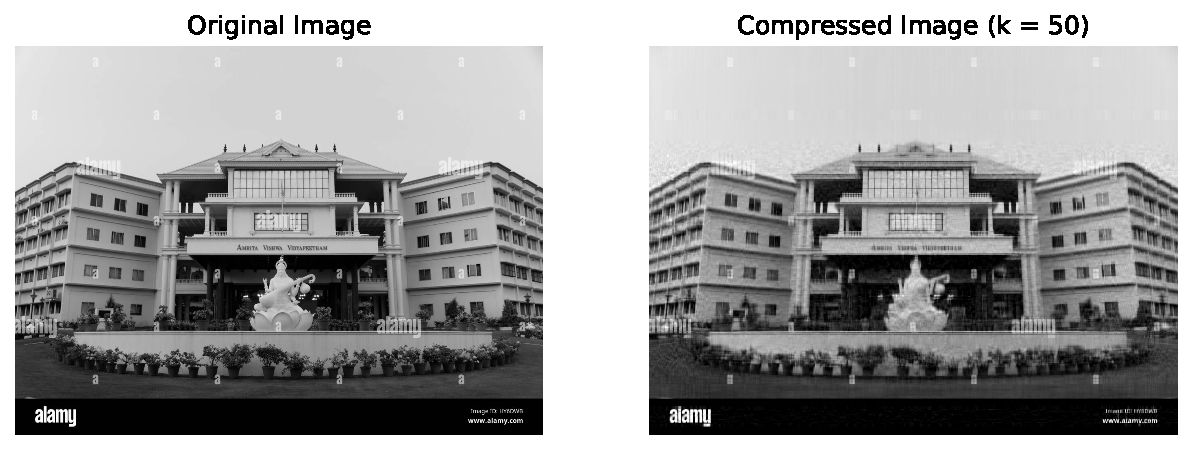
\includegraphics{index_files/figure-pdf/cell-2-output-1.pdf}

To assess the quality of the original and compressed images, various
metrics can be employed. Two common measures are Peak Signal-to-Noise
Ratio (PSNR) and Mean Squared Error (MSE).

The Mean Squared Error quantifies the average squared difference between
pixel values of the original and compressed images. It is defined as:

\[
\text{MSE} = \frac{1}{m \cdot n} \sum_{i=1}^{m} \sum_{j=1}^{n} (A(i,j) - A_k(i,j))^2
\]

where \(m\) and \(n\) are the dimensions of the image, \(A(i,j)\) is the
pixel value of the original image, and \(A_k(i,j)\) is the pixel value
of the compressed image.

The Peak Signal-to-Noise Ratio (PSNR) is a measure that compares the
maximum possible power of a signal to the power of corrupting noise that
affects the fidelity of its representation. It is given by:

\[
\text{PSNR} = 10 \cdot \log_{10}\left(\frac{M_{\text{AX}}^2}{\text{MSE}}\right)
\]

where \(M_{\text{AX}}\) is the maximum pixel value, typically 255 for an
8-bit image.

Below is the additional MATLAB code to calculate MSE and PSNR:

\subsubsection{Code}

\begin{Shaded}
\begin{Highlighting}[]
\CommentTok{\% Calculate Mean Squared Error (MSE)}
\VariableTok{mse} \OperatorTok{=} \VariableTok{mean}\NormalTok{((}\VariableTok{A}\NormalTok{(}\OperatorTok{:}\NormalTok{) }\OperatorTok{{-}} \VariableTok{A\_k}\NormalTok{(}\OperatorTok{:}\NormalTok{))}\OperatorTok{.\^{}}\FloatTok{2}\NormalTok{)}\OperatorTok{;}

\CommentTok{\% Calculate Peak Signal{-}to{-}Noise Ratio (PSNR)}
\VariableTok{max\_pixel\_value} \OperatorTok{=} \FloatTok{255}\OperatorTok{;} \CommentTok{\% Maximum pixel value for 8{-}bit images}
\VariableTok{psnr} \OperatorTok{=} \FloatTok{10} \OperatorTok{*} \VariableTok{log10}\NormalTok{((}\VariableTok{max\_pixel\_value}\OperatorTok{\^{}}\FloatTok{2}\NormalTok{) }\OperatorTok{/} \VariableTok{mse}\NormalTok{)}\OperatorTok{;}

\CommentTok{\% Calculate sizes}
\VariableTok{original\_size} \OperatorTok{=} \VariableTok{numel}\NormalTok{(}\VariableTok{A}\NormalTok{) }\OperatorTok{*} \FloatTok{8}\OperatorTok{;} \CommentTok{\% Size of the original image in bytes (double data type)}
\VariableTok{compressed\_size} \OperatorTok{=}\NormalTok{ (}\VariableTok{k} \OperatorTok{*}\NormalTok{ (}\VariableTok{size}\NormalTok{(}\VariableTok{A}\OperatorTok{,} \FloatTok{1}\NormalTok{) }\OperatorTok{+} \VariableTok{size}\NormalTok{(}\VariableTok{A}\OperatorTok{,} \FloatTok{2}\NormalTok{))) }\OperatorTok{*} \FloatTok{8}\OperatorTok{;} \CommentTok{\% Size of compressed representation (U, S\_k, V)}

\CommentTok{\% Display results}
\VariableTok{fprintf}\NormalTok{(}\SpecialStringTok{\textquotesingle{}Mean Squared Error (MSE): \%.4f\textbackslash{}n\textquotesingle{}}\OperatorTok{,} \VariableTok{mse}\NormalTok{)}\OperatorTok{;}
\VariableTok{fprintf}\NormalTok{(}\SpecialStringTok{\textquotesingle{}Peak Signal{-}to{-}Noise Ratio (PSNR): \%.4f dB\textbackslash{}n\textquotesingle{}}\OperatorTok{,} \VariableTok{psnr}\NormalTok{)}\OperatorTok{;}
\VariableTok{fprintf}\NormalTok{(}\SpecialStringTok{\textquotesingle{}Original Image Size: \%.2f KB\textbackslash{}n\textquotesingle{}}\OperatorTok{,} \VariableTok{original\_size} \OperatorTok{/} \FloatTok{1024}\NormalTok{)}\OperatorTok{;} \CommentTok{\% Convert to KB}
\VariableTok{fprintf}\NormalTok{(}\SpecialStringTok{\textquotesingle{}Compressed Image Size: \%.2f KB\textbackslash{}n\textquotesingle{}}\OperatorTok{,} \VariableTok{compressed\_size} \OperatorTok{/} \FloatTok{1024}\NormalTok{)}\OperatorTok{;} \CommentTok{\% Convert to KB}
\VariableTok{fprintf}\NormalTok{(}\SpecialStringTok{\textquotesingle{}Size Reduction: \%.2f KB\textbackslash{}n\textquotesingle{}}\OperatorTok{,}\NormalTok{ (}\VariableTok{original\_size} \OperatorTok{{-}} \VariableTok{compressed\_size}\NormalTok{) }\OperatorTok{/} \FloatTok{1024}\NormalTok{)}\OperatorTok{;} \CommentTok{\% Convert to KB}
\end{Highlighting}
\end{Shaded}

\subsubsection{Output}

\begin{verbatim}
Mean Squared Error (MSE): 110.2853
Peak Signal-to-Noise Ratio (PSNR): 27.7056 dB
Original Image Size: 9709.38 KB
Compressed Image Size: 900.78 KB
Size Reduction: 8808.59 KB
\end{verbatim}

\phantomsection\label{refs}
\begin{CSLReferences}{0}{0}
\bibitem[\citeproctext]{ref-Chen2018SingularVD}
\CSLLeftMargin{{[}1{]} }%
\CSLRightInline{Z. Chen, {``Singular value decomposition and its
applications in image processing,''} \emph{Proceedings of the 2018 1st
International Conference on Mathematics and Statistics}, 2018
{[}Online{]}. Available:
\url{https://api.semanticscholar.org/CorpusID:53245257}}

\bibitem[\citeproctext]{ref-cao2006singular}
\CSLLeftMargin{{[}2{]} }%
\CSLRightInline{L. Cao, {``Singular value decomposition applied to
digital image processing,''} \emph{Division of Computing Studies,
Arizona State University Polytechnic Campus, Mesa, Arizona State
University polytechnic Campus}, pp. 1--15, 2006. }

\end{CSLReferences}


% Can use something like this to put references on a page
% by themselves when using endfloat and the captionsoff option.
\ifCLASSOPTIONcaptionsoff
  \newpage
\fi

% trigger a \newpage just before the given reference
% number - used to balance the columns on the last page
% adjust value as needed - may need to be readjusted if
% the document is modified later
%\IEEEtriggeratref{8}
% The "triggered" command can be changed if desired:
%\IEEEtriggercmd{\enlargethispage{-5in}}

% Uncomment when use biblatex with style=ieee
%\renewcommand{\bibfont}{\footnotesize} % for IEEE bibfont size

\pagebreak[3]
\begin{IEEEbiography}[\includegraphics{david-folio.png}]{Siju K S}
Use \texttt{IEEEbiography} with figure as option and the author name as
the argument followed by the biography text.
\end{IEEEbiography}
\begin{IEEEbiographynophoto}{John Doe}
Use \texttt{IEEEbiographynophoto} and the author name as the argument
followed by the biography text.
\end{IEEEbiographynophoto}
% that's all folks
\end{document}

